%=======================================================================
%  Póster A0 vertical — Proyectos REDD+ y deforestación municipal en
%  Colombia: un diseño escalonado con intensidad de tratamiento, 2001–2024
%
%  Compilar:  pdflatex poster.tex   (dos pasadas)
%  Requiere:  beamerposter, pgfplots, booktabs, tcolorbox
%  Figuras (copiar desde outputs/figuras/ a la carpeta del .tex):
%     44_event_study_base_universal.png (44_honestdid.R)
%     43_leave_one_out.png              (43_robustez_anticipacion_y_loo.R)
%     42_dosis_vs_att_relativo.png      (42_pendiente_dosis_manual.R)
%=======================================================================
\documentclass[final,t]{beamer}
\usepackage[orientation=portrait,size=a0,scale=0.97]{beamerposter}
\usepackage[utf8]{inputenc}
\usepackage[T1]{fontenc}
\usepackage{helvet}
\renewcommand{\familydefault}{\sfdefault}
\usepackage{anyfontsize}
\usepackage{colortbl}
\usepackage{booktabs}
\usepackage{tabularx}
\usepackage{ragged2e}
\usepackage{amsmath}
\usepackage{graphicx}
\usepackage{tcolorbox}
\usepackage{pgfplots}
\pgfplotsset{compat=1.18}
\tcbuselibrary{skins}

%----------------------- Paleta -----------------------
\definecolor{tinta}{HTML}{12261E}
\definecolor{dosel}{HTML}{1D4F3F}
\definecolor{papel}{HTML}{F2F4EF}
\definecolor{reduccion}{HTML}{2F7A5B}
\definecolor{brasa}{HTML}{8F3B1F}
\definecolor{amazonia}{HTML}{B8860F}
\definecolor{regla}{HTML}{C4CEC6}
\definecolor{tenue}{HTML}{5B6E63}
\definecolor{cajafondo}{HTML}{E6EBE4}
\definecolor{alertafondo}{HTML}{F4E7E0}
\definecolor{politicafondo}{HTML}{E4EFE7}
\definecolor{orofondo}{HTML}{F6ECD2}

%----------------------- Tema -------------------------
\usetheme{default}
\usecolortheme{default}
\setbeamercolor{background canvas}{bg=papel}
\setbeamercolor{normal text}{fg=tinta}
\setbeamercolor{block title}{bg=papel,fg=dosel}
\setbeamercolor{block body}{bg=papel,fg=tinta}
\setbeamerfont{block title}{series=\bfseries,size=\Large}
\setbeamertemplate{navigation symbols}{}
\setbeamertemplate{caption}[numbered]
\setbeamerfont{caption}{size=\small}
\setbeamercolor{caption name}{fg=tenue}
\setbeamercolor{itemize item}{fg=reduccion}
\setbeamertemplate{itemize item}{\raisebox{0.18ex}{\rule{0.45ex}{0.45ex}}}
\setlength{\parskip}{0.4\baselineskip}

% Título de sección con filete y referencia al capítulo de la tesis
\newcommand{\seccion}[2]{%
  \par\vspace{0.5\baselineskip}%
  {\color{dosel}\Large\bfseries #1\hfill{\color{tenue}\normalsize\mdseries #2}}\par
  \vspace{-0.35\baselineskip}%
  {\color{dosel}\rule{\linewidth}{2.2pt}}\par
  \vspace{0.25\baselineskip}%
}

% Nota de pie, cuerpo pequeño
\newcommand{\nota}[1]{{\color{tenue}\small #1\par}}

% Cifra destacada
\newcommand{\cifra}[2]{%
  \parbox[t]{0.46\linewidth}{%
    {\color{tinta}\rule{\linewidth}{2.5pt}}\\[0.25\baselineskip]
    {\color{dosel}\fontsize{50}{52}\selectfont\bfseries #1}\\[0.2\baselineskip]
    {\color{tenue}\small #2}}%
}

% Caja de contenido
\newtcolorbox{caja}[2][cajafondo]{
  colback=#1, colframe=dosel, boxrule=0pt, leftrule=5pt,
  sharp corners, left=8pt, right=8pt, top=8pt, bottom=8pt,
  title=\textbf{#2}, coltitle=tinta, fonttitle=\large,
  attach title to upper=\par\vspace{2mm}
}

\begin{document}
\begin{frame}[t]{}

%=======================================================================
%  CABECERA
%=======================================================================
\begin{tcolorbox}[colback=dosel,colframe=dosel,boxrule=0pt,sharp corners,
  left=1.2cm,right=1.2cm,top=1.0cm,bottom=1.0cm]
  {\color{papel!70}\normalsize Maestría en Economía Aplicada \quad\textbullet\quad Tesis de grado
   \hfill Entidad destinataria: Ministerio de Ambiente y Desarrollo Sostenible (MADS)}\\[0.3cm]
  {\color{papel!40}\rule{\linewidth}{1pt}}\\[0.6cm]
  {\color{papel}\fontsize{72}{80}\selectfont\bfseries
   Proyectos REDD+ y deforestación municipal en Colombia:}\\[0.35cm]
  {\color{papel!80}\fontsize{50}{58}\selectfont\bfseries
   un diseño escalonado con intensidad de tratamiento, 2001--2024}\\[0.7cm]
  {\color{papel!85}\large\textbf{José David Cuervo Urrego}\quad\textbullet\quad
   \textbf{Harold Stiven Acuña Alaguna}\qquad Asesor: Jorge Luis Montero Mestre}
\end{tcolorbox}



%=======================================================================
%  FRANJA: HALLAZGO PRINCIPAL
%=======================================================================
\begin{tcolorbox}[colback=tinta,colframe=tinta,boxrule=0pt,sharp corners,
  left=1.2cm,right=1.2cm,top=0.9cm,bottom=0.9cm]
\begin{minipage}[c]{0.36\linewidth}
  {\color{papel}\fontsize{40}{46}\selectfont\bfseries El signo resiste; la magnitud no}\\[0.6cm]
  \setlength{\leftskip}{0.9cm}\setlength{\parindent}{-0.9cm}
  \color{papel!75}\large
  \textcolor{amazonia}{\rule{0.45ex}{0.45ex}}\hspace{0.5cm}Negativo en todas las especificaciones,
  pero \textbf{\textcolor{amazonia}{ningún intervalo excluye el cero}}.\par\vspace{0.35cm}
  \textcolor{amazonia}{\rule{0.45ex}{0.45ex}}\hspace{0.5cm}Con base $g-2$ en lugar de $g-1$ el efecto cae
  \textbf{\textcolor{amazonia}{60\,\%}}: un salto de deforestación el año previo a la adopción
  se lee como efecto (reversión a la media).\par\vspace{0.35cm}
  \textcolor{amazonia}{\rule{0.45ex}{0.45ex}}\hspace{0.5cm}Ninguna exclusión individual cambia el signo,
  pero \textbf{\textcolor{amazonia}{tres de 37 municipios}} sostienen casi todo el estimado puntual.\par
\end{minipage}\hfill
\begin{minipage}[c]{0.60\linewidth}
\centering
\begin{tikzpicture}[x=0.0195cm,y=1cm,
   nombre/.style={anchor=east,align=right,text width=12.5cm,text=papel!75,font=\normalsize},
   sub/.style={anchor=east,align=right,text width=12.5cm,text=papel!50,font=\small},
   valor/.style={anchor=south,font=\bfseries\normalsize},
   eje/.style={anchor=north,text=papel!50,font=\normalsize}]

  % rejilla vertical
  \foreach \v in {-1000,-750,-500,-250,250}
    \draw[papel!22,very thin] (\v,0.95) -- (\v,-9.05);
  \draw[papel!65,dashed,semithick] (0,1.15) -- (0,-9.25);

  % --- Principal, base g-1 ---
  \node[nombre] at (-1120,0) {Especificación principal};
  \node[sub]    at (-1120,-0.85) {base $g-1$};
  \draw[amazonia,thick] (-1029.25,0) -- (99.47,0);
  \fill[amazonia] (-464.89,-0.35) rectangle (0,0.35);
  \node[valor,text=amazonia!60] at (-232,0.42) {$-$464{,}9};

  % --- base g-2 ---
  \node[nombre] at (-1120,-2) {Año base anterior};
  \node[sub]    at (-1120,-2.85) {base $g-2$};
  \draw[reduccion!80,semithick] (-654.93,-2) -- (285.78,-2);
  \fill[reduccion!85] (-184.58,-2.35) rectangle (0,-1.65);
  \node[valor,text=reduccion!45] at (-92,-1.58) {$-$184{,}6};

  % --- base g-3 ---
  \node[nombre] at (-1120,-4) {Año base anterior};
  \node[sub]    at (-1120,-4.85) {base $g-3$};
  \draw[reduccion!80,semithick] (-923.51,-4) -- (355.98,-4);
  \fill[reduccion!85] (-283.77,-4.35) rectangle (0,-3.65);
  \node[valor,text=reduccion!45] at (-142,-3.58) {$-$283{,}8};

  % --- sin Cartagena del Chaira ---
  \node[nombre] at (-1120,-6) {Sin Cartagena del Chairá};
  \node[sub]    at (-1120,-6.85) {1 de 37 tratados};
  \draw[reduccion!80,semithick] (-737.15,-6) -- (206.45,-6);
  \fill[reduccion!85] (-265.35,-6.35) rectangle (0,-5.65);
  \node[valor,text=reduccion!45] at (-133,-5.58) {$-$265{,}4};

  % --- sin los 3 mas influyentes ---
  \node[nombre] at (-1120,-8) {Sin los tres más influyentes};
  \node[sub]    at (-1120,-8.85) {prueba de estrés, ver Fig.~6.2};
  \draw[papel!55,semithick] (-466.43,-8) -- (452.11,-8);
  \fill[papel!55] (-7.16,-8.35) rectangle (0,-7.65);
  \node[valor,text=papel!60] at (-60,-7.58) {$-$7{,}2};

  % --- escala ---
  \foreach \v/\t in {-1000/$-$1.000,-750/$-$750,-500/$-$500,-250/$-$250,0/0,250/$+$250}
    \node[eje] at (\v,-9.35) {\t};
  \node[anchor=north,text=papel!50,font=\normalsize] at (-300,-10.15)
    {ATT balanceado $e=0,\dots,5$ sobre pérdida anual de bosque (ha) \textbullet\ línea = IC 95\,\%};
\end{tikzpicture}
\end{minipage}
\end{tcolorbox}



%=======================================================================
%  TRES COLUMNAS
%=======================================================================
\begin{columns}[t]

%-------------------- COLUMNA 1 --------------------
\begin{column}{0.305\paperwidth}
\justifying

\seccion{Problema de política}{}
\begin{itemize}
  \item El mecanismo de no causación (Ley 1819 de 2016; Decreto 926 de 2017) permite compensar
        el impuesto al carbono con créditos certificados.
  \item Ese incentivo aceleró la expansión de proyectos REDD+ sin evaluación causal previa.
  \item[\textcolor{brasa}{\rule{0.45ex}{0.45ex}}] Sobreacreditación documentada: los créditos emitidos
        equivalen a \textbf{10,7 veces} las reducciones verificables en 44 proyectos REDD+
        (Swinfield et al., 2026).
  \item Sin evidencia causal, el MADS no distingue beneficio climático real de acreditación
        no atribuible.
\end{itemize}

\vspace{0.3cm}
{\color{amazonia}\rule{3pt}{2.6cm}}\hspace{0.4cm}%
\begin{minipage}[b]{0.88\linewidth}
  {\color{dosel}\fontsize{30}{36}\selectfont\itshape
   ¿Cuál es el efecto causal de la implementación de proyectos REDD+ sobre la
   deforestación en los municipios colombianos?}
\end{minipage}

\vspace{0.3cm}
\nota{Se evalúa la \textbf{intervención territorial}, no el crédito ni la certificación: bonos de
carbono no es sinónimo de REDD+. Ninguno de los 12 proyectos de Gold Standard en Colombia es
REDD+, y de los REDD+ de Verra solo 13 están registrados.}

\seccion{Datos}{}
\cifra{1.122}{municipios}\hfill\cifra{26.928}{observaciones municipio--año}

\vspace{0.5cm}
\cifra{43}{municipios tratados REDD+ (depurado)}\hfill\cifra{37}{tratados en la ventana de cohortes 2013--2019}

\vspace{0.3cm}
\textbf{\large Resultado}
\begin{itemize}
  \item Pérdida de cobertura arbórea, Global Forest Change a 30~m (Hansen et al., 2013),
        por estadística zonal.
  \item Distribución muy asimétrica: mediana de 22~ha frente a máximos sobre 30.000~ha
        $\rightarrow$ se reporta también el efecto \textbf{relativo} a la deforestación
        propia de 2001--2012.
\end{itemize}

\textbf{\large Tratamiento}
\nota{Registros consultados y método de asignación municipal.}
\begin{center}
\begin{tabularx}{\linewidth}{Xrl}
\toprule
\rowcolor{dosel}
\textcolor{papel}{\textbf{Registro}} & \textcolor{papel}{\textbf{Proy.}} &
\textcolor{papel}{\textbf{Asignación}}\\
\midrule
Verra (API Platts/S\&P) & 101 & Punto en polígono\\
Gold Standard (API)     & 28  & Punto en polígono\\
RENARE (MADS)           & 281 & Coincidencia textual\\
Cercarbono (Excel)      & 234 & Coincidencia textual\\
OffsetsDB               & 270 & Solo descubrimiento\\
\bottomrule
\end{tabularx}
\end{center}
\nota{Filtro REDD+ por campo estructurado (metodologías VM0006, VM0007, VM0009, VM0015 y actividad
AFOLU), no por nombre del proyecto: 82 eventos en 50 municipios.}

\begin{caja}{Depuración del tratamiento}
\begin{itemize}
  \item \textbf{Geocodificación:} se excluye CO2ROZO, 400.000~ha ubicadas en la sede del proponente
        (Barranquilla).
  \item \textbf{Estado de registro:} 6 municipios cuyo único vínculo REDD+ es un proyecto
        retirado o rechazado salen de la muestra; \textbf{no pasan a control}.
  \item La cohorte la fija el proyecto vivo: Mitú pasa de 2017 a 2018.
  \item[\textcolor{amazonia}{\rule{0.45ex}{0.45ex}}] De 48 a 43 tratados. El ATT se mueve 9\,\%:
        el resultado es robusto a la depuración.
\end{itemize}
\end{caja}

\seccion{Hipótesis y contraste}{}
\begin{center}
\begin{tabularx}{\linewidth}{lX}
\toprule
\rowcolor{dosel}
\textcolor{papel}{\textbf{Hipótesis}} & \textcolor{papel}{\textbf{Veredicto empírico}}\\
\midrule
H1. ATT negativo           & Signo consistente; ningún IC excluye el cero\\
H2. Sin dinámicas previas  & $g-1$ es un año alto: 40--60\,\% del estimado depende de la base;
                             $\bar{M}$ de ruptura $=0$\\
H3. Efecto persistente     & Sin precisión para afirmarlo\\
H4. Fuga hacia vecinos     & Sin fuga detectable: $-$59~ha, IC [$-$221 ; 102] (DR, 108 vecinos expuestos)\\
H5. Mayor efecto a mayor intensidad & Sin gradiente identificable\\
\bottomrule
\end{tabularx}
\end{center}

\end{column}

%-------------------- COLUMNA 2 --------------------
\begin{column}{0.305\paperwidth}
\justifying

\seccion{Estrategia empírica}{}
\nota{Diferencias en diferencias con adopción escalonada (Callaway y Sant'Anna, 2021),
identificado contra el año previo a la adopción:}
\begin{tcolorbox}[colback=cajafondo,colframe=regla,boxrule=0.8pt,sharp corners]
\centering
\[
  ATT(g,t) \;=\; \mathbb{E}\!\left[Y_{t}-Y_{g-1}\,\middle|\,G_{g}=1\right]
               \;-\; \mathbb{E}\!\left[Y_{t}-Y_{g-1}\,\middle|\,C=1\right]
\]
\raggedright\nota{$G_g$: cohorte que adopta en el año $g$. $C$: municipios aún no tratados.}
\end{tcolorbox}

\nota{Intensidad de tratamiento continua (Callaway, Goodman-Bacon y Sant'Anna, 2024):}
\begin{tcolorbox}[colback=cajafondo,colframe=regla,boxrule=0.8pt,sharp corners]
\centering
\[
  ATT(d) \;=\; \mathbb{E}\!\left[\Delta Y \,\middle|\, D=d\right]
         \;-\; \mathbb{E}\!\left[\Delta Y \,\middle|\, D=0\right]
\]
\raggedright\nota{La pendiente $\partial ATT(d)/\partial d$ solo es causal bajo tendencias
paralelas \emph{fuertes}: que municipios de distinta dosis respondan igual a la misma dosis.}
\end{tcolorbox}

\begin{itemize}
  \item Doblemente robusto con \textbf{diez covariables} de línea base: clima, accesibilidad,
        conflicto, coca, deforestación previa y su tendencia.
  \item Cohortes 2013--2019; los tratados fuera de la ventana salen de la muestra.
  \item Robustez: año base (anticipación), exclusión uno a uno, D1 sin depurar y
        sensibilidad de Rambachan y Roth (2023) a violaciones de tendencias paralelas.
\end{itemize}

\seccion{Efecto promedio}{}
\nota{Tabla 6.1. ATT simple sobre la pérdida de bosque, cohortes 2013--2019. Relativo: ATT sobre
la media pretratamiento de los tratados.}
\begin{center}
\begin{tabularx}{\linewidth}{Xrrr}
\toprule
\rowcolor{dosel}
\textcolor{papel}{\textbf{Especificación}} & \textcolor{papel}{\textbf{ATT (ha)}} &
\textcolor{papel}{\textbf{EE}} & \textcolor{papel}{\textbf{Rel.}}\\
\midrule
\rowcolor{orofondo}
\textbf{Depurada · DR (principal)} & \textcolor{reduccion}{\textbf{$-$424,99}} & 263,82 & $-$43\,\%\\
Depurada · sin covariables & \textcolor{reduccion}{\textbf{$-$176,87}} & 298,25 & $-$18\,\%\\
Sin depurar · DR           & \textcolor{reduccion}{\textbf{$-$388,61}} & 208,43 & $-$39\,\%\\
\bottomrule
\end{tabularx}
\end{center}
\begin{itemize}
  \item IC 95\,\% de la principal: [$-$942 ; 92] ha.
  \item[\textcolor{brasa}{\rule{0.45ex}{0.45ex}}] Sin covariables el efecto cae a menos de la mitad:
        la comparación incondicional contra el promedio nacional es débil.
\end{itemize}

\seccion{Año base y tendencias previas}{}
\begin{center}
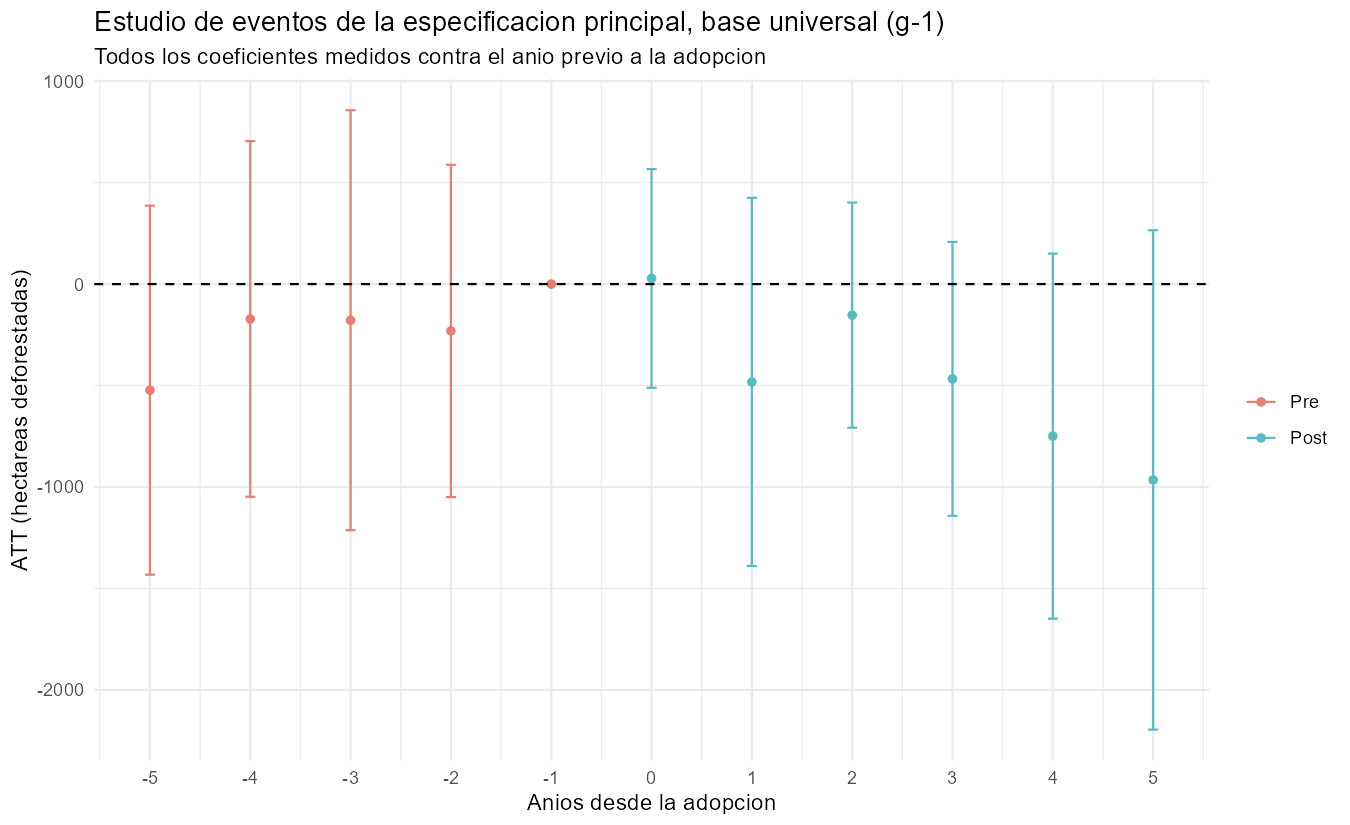
\includegraphics[width=0.92\linewidth]{44_event_study_base_universal.png}
\end{center}
\nota{Figura 6.1. Estudio de eventos de la especificación principal, todos los coeficientes contra
$g-1$ (base universal).}
\begin{itemize}
  \item Los cuatro coeficientes previos son negativos ($-$172 a $-$523~ha): \textbf{$g-1$ es un año
        alto}. Contra el promedio previo, el efecto post es $\approx -$189~ha, en línea con las
        bases $g-2$ y $g-3$ ($-$185 y $-$284~ha).
  \item[\textcolor{amazonia}{\rule{0.45ex}{0.45ex}}] Rambachan y Roth: \textbf{$\bar{M}$ de ruptura
        $=0$}, porque el intervalo convencional ya incluye el cero. Con $\bar{M}=1$, el IC del
        promedio $e=0\dots5$ se abre a [$-$3.593 ; 2.013]~ha.
\end{itemize}

\seccion{Influencia por municipio}{}
\begin{center}
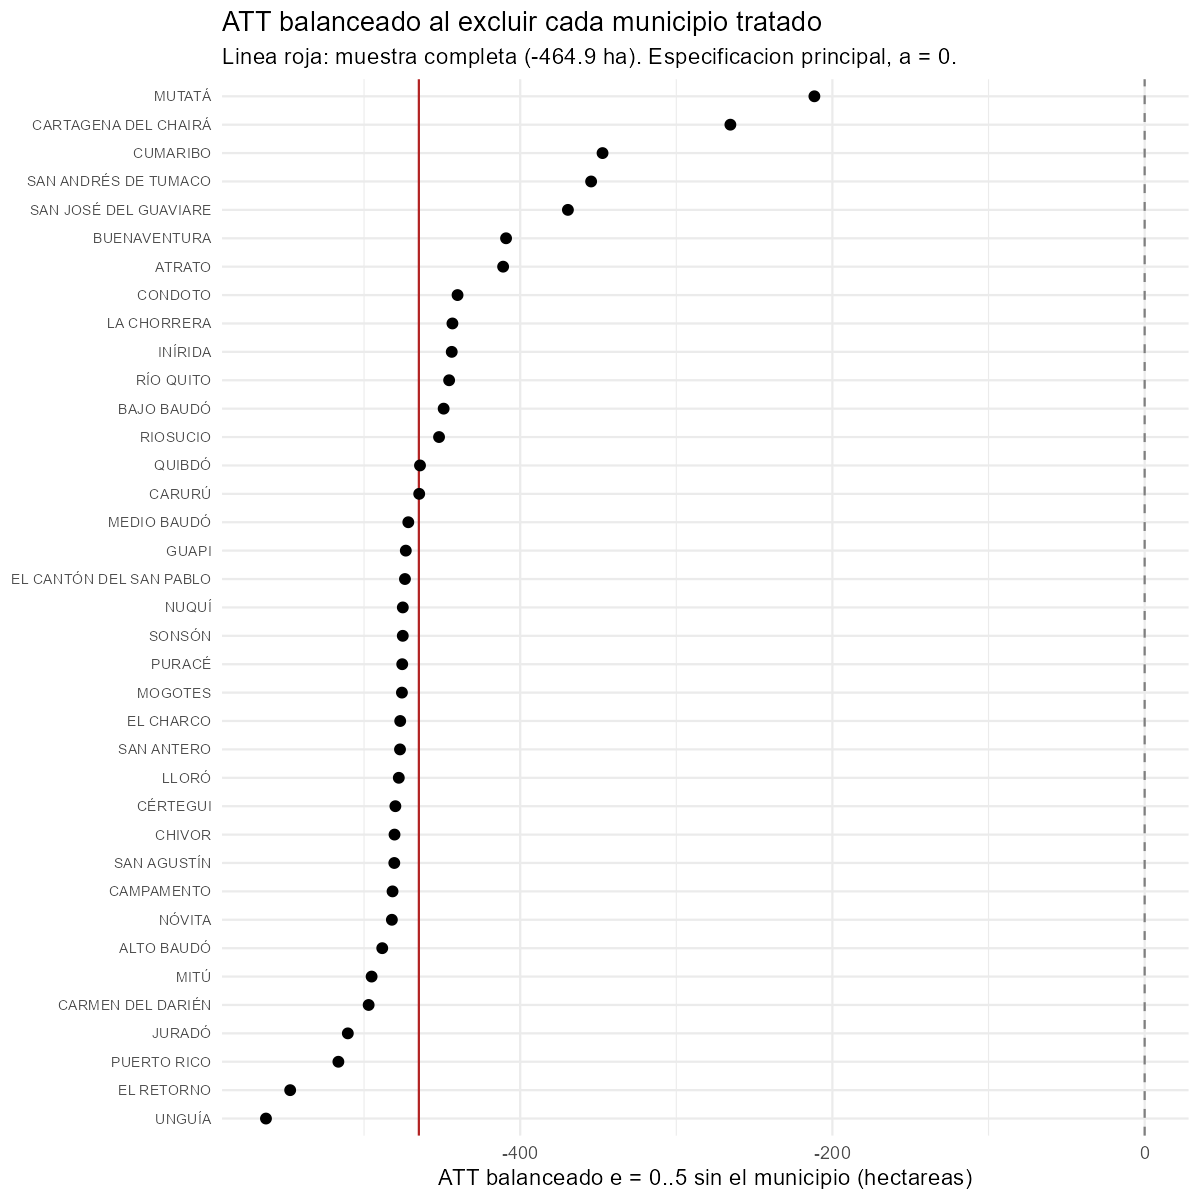
\includegraphics[width=0.60\linewidth]{43_leave_one_out.png}
\end{center}
\nota{Figura 6.2. ATT balanceado al excluir cada uno de los 37 tratados. Rango: [$-$563 ; $-$212]~ha.}

\end{column}

%-------------------- COLUMNA 3 --------------------
\begin{column}{0.305\paperwidth}
\justifying

\seccion{Intensidad del tratamiento}{}
\nota{Dos medidas pedidas por la dirección, con área declarada del proyecto $a_p$ y bosque base
$F_i^{2000}$ (dosel $\geq$30\,\%, validado contra Earth Engine):}
\begin{tcolorbox}[colback=cajafondo,colframe=regla,boxrule=0.8pt,sharp corners]
\centering
\[
  D_i^{\text{área}} = \frac{\sum_{p\in P_i} a_p}{A_i}
  \qquad\qquad
  D_i^{\text{bosque}} = \frac{\sum_{p\in P_i} a_p}{F_i^{2000}}
\]
\end{tcolorbox}
\cifra{29 de 43}{tratados con área publicada}\hfill\cifra{0,97}{correlación entre las dos medidas}

\vspace{0.2cm}
\nota{Tabla 6.5. ATT por tercil de $D^{\text{bosque}}$, estudio de eventos balanceado, relativo a la
media pretratamiento de cada tercil.}
\begin{center}
\begin{tabularx}{\linewidth}{Xrrrr}
\toprule
\rowcolor{dosel}
\textcolor{papel}{\textbf{Tercil}} & \textcolor{papel}{\textbf{$n$}} &
\textcolor{papel}{\textbf{Media pre}} & \textcolor{papel}{\textbf{Sin cov.}} &
\textcolor{papel}{\textbf{DR}}\\
\midrule
Bajo  & 9 & 2.191~ha & $-$28\,\% & $-$41\,\%\\
Medio & 9 &   522~ha & $+$8\,\%  & $-$7\,\%\\
Alto  & 7 &   114~ha & $-$33\,\% & $-$1\,\%\\
\bottomrule
\end{tabularx}
\end{center}
\nota{En hectáreas, el tercil bajo parecía el más efectivo: su deforestación base es 19 veces la
del alto. Normalizado, no hay gradiente monótono.}

\begin{center}
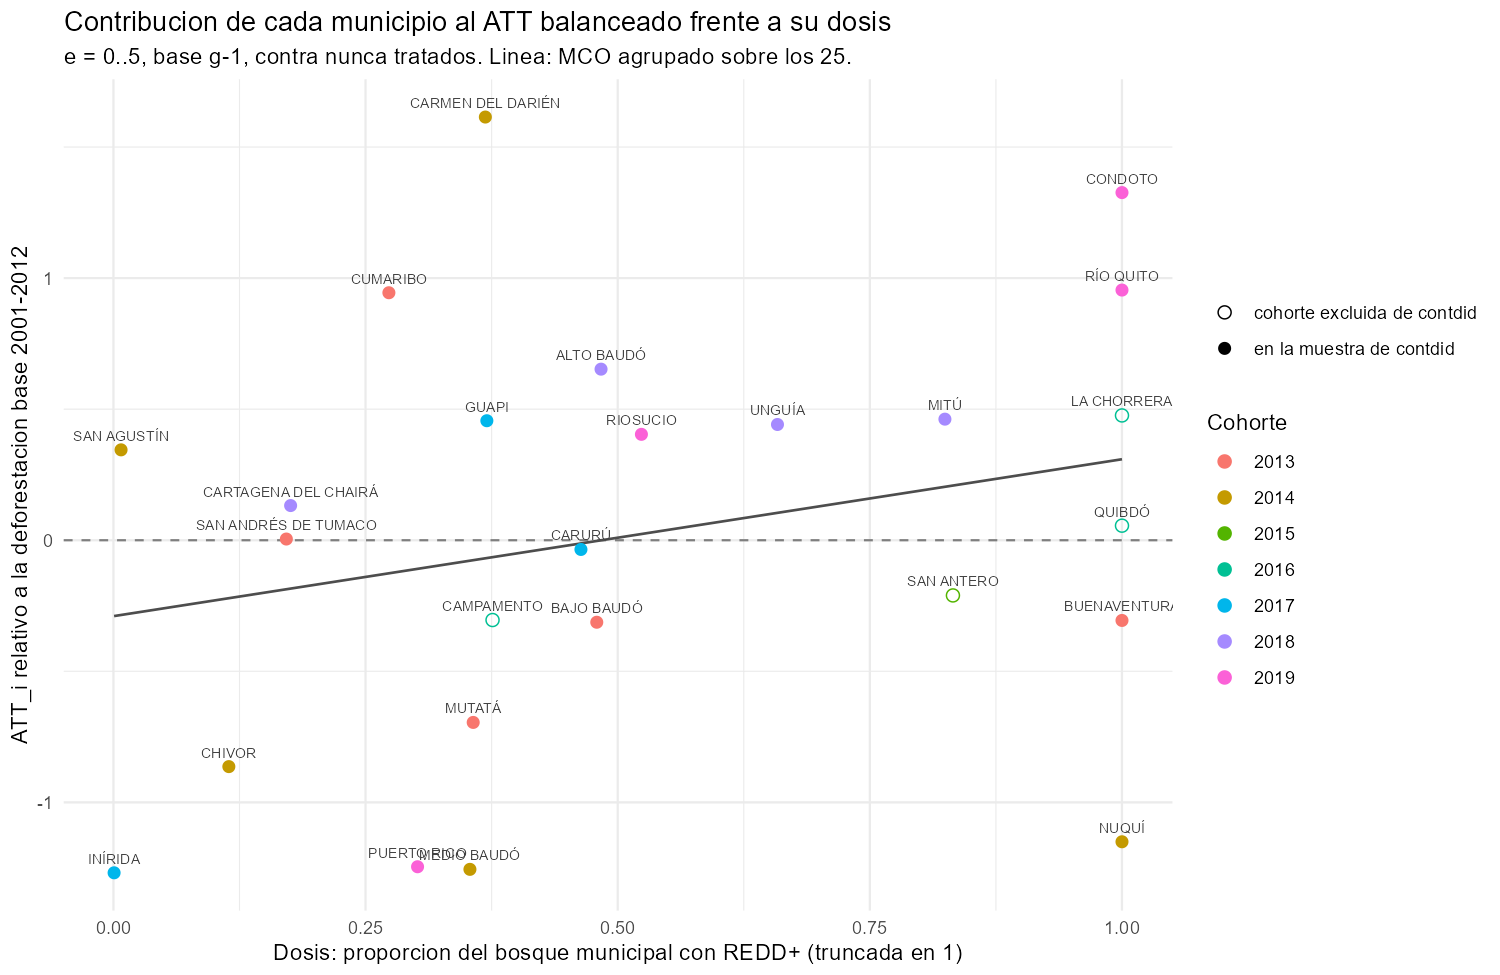
\includegraphics[width=0.96\linewidth]{42_dosis_vs_att_relativo.png}
\end{center}
\nota{Figura 6.3. Contribución de cada municipio al ATT frente a su dosis, escala relativa.}

\begin{center}
\begin{tabularx}{\linewidth}{Xrl}
\toprule
\rowcolor{dosel}
\textcolor{papel}{\textbf{Pendiente}} & \textcolor{papel}{\textbf{Punto}} &
\textcolor{papel}{\textbf{Inferencia}}\\
\midrule
\textit{contdid} 0.1.1       & 0,76     & EE 0,0009: subestimado\\
Manual, base $g-1$           & 0,60     & IC [$-$0,20 ; 1,39]; $p$ = 0,22\\
Manual, base $g-5\dots g-1$  & $-$0,05  & cambia de signo\\
\bottomrule
\end{tabularx}
\end{center}
\nota{Descomposición exacta del ATT por municipio; bootstrap estratificado de tratados y controles,
y permutación de la dosis.}

\begin{caja}[alertafondo]{Por qué no hay curva dosis-respuesta}
\begin{itemize}
  \item Entre 21 y 25 municipios con variación de dosis suficiente.
  \item Un tercio de las dosis \textbf{censuradas en 1}: los proyectos grandes cruzan fronteras
        municipales y el área declarada excede la del municipio anfitrión.
  \item La pendiente depende del año base: no está identificada.
\end{itemize}
\end{caja}

\begin{caja}[orofondo]{El salto previo tiene lectura de política}
Si los proyectos se instalan tras un pico de deforestación, el DiD atribuye al proyecto el retorno
a la normalidad, y la línea base del proyecto incorpora ese pico e infla los créditos. Es el
mecanismo de sobreacreditación documentado para REDD+ voluntario (West et al., 2020; 2023): el
sesgo que complica la identificación es el mismo que compromete la integridad de los créditos.
El salto previo aparece también en los municipios vecinos: la presión es regional.
\end{caja}

\seccion{Limitaciones}{}
\begin{itemize}
  \item[\textcolor{brasa}{\rule{0.45ex}{0.45ex}}] Sin polígonos: la dosis suma áreas declaradas
        (no su unión) y las asigna al municipio anfitrión.
  \item[\textcolor{brasa}{\rule{0.45ex}{0.45ex}}] Cercarbono y RENARE no publican área ni estado de
        registro: 14 tratados sin dosis.
  \item[\textcolor{brasa}{\rule{0.45ex}{0.45ex}}] Se mide pérdida de cobertura arbórea, no de bosque
        natural; la salida de las FARC-EP desde 2016 es explicación alternativa en la Amazonía.
\end{itemize}

\seccion{Implicaciones para el MADS}{}
\begin{caja}[politicafondo]{}
\begin{itemize}
  \item \textbf{MRV.} Exigir polígonos georreferenciados en RENARE: sin ellos no se evalúan
        intensidad ni fuga.
  \item \textbf{Líneas base.} Verificar que no incorporen picos recientes de deforestación.
  \item \textbf{Registro.} Distinguir proyectos vivos, retirados y rechazados; la evidencia no
        respalda una acreditación uniforme.
\end{itemize}
\end{caja}

\end{column}
\end{columns}

\vfill

%=======================================================================
%  PIE
%=======================================================================
\colorbox{tinta}{%
\begin{minipage}[t]{\dimexpr\paperwidth-2.4cm\relax}
\vspace{0.7cm}
\hspace{0.8cm}%
\begin{minipage}[t]{0.63\linewidth}
  {\color{papel!65}\small\textbf{\color{papel}Referencias principales.}
  Callaway y Sant'Anna (2021) \textbullet\ Callaway, Goodman-Bacon y Sant'Anna (2024)
  \textbullet\ Sun y Abraham (2021) \textbullet\ Goodman-Bacon (2021)
  \textbullet\ Rambachan y Roth (2023) \textbullet\ Ashenfelter (1978) \textbullet\ Hansen et al. (2013)
  \textbullet\ West et al. (2020, 2023) \textbullet\ Guizar-Coutiño et al. (2022)
  \textbullet\ Swinfield et al. (2026) \textbullet\ Probst et al. (2024).}
\end{minipage}\hfill
\begin{minipage}[t]{0.32\linewidth}
  {\color{papel!65}\small\textbf{\color{papel}Reproducibilidad.}
  Panel en Python (pandas, GeoPandas, Google Earth Engine); estimación en R
  (\textit{did}, \textit{contdid} 0.1.1, \textit{HonestDiD}, \textit{spdep}).}
\end{minipage}
\hspace{0.8cm}
\vspace{0.7cm}
\end{minipage}}

\end{frame}
\end{document}
